\documentclass[stu,12pt,floatsintext]{apa7}
\usepackage[american]{babel}
\usepackage{csquotes} % One of the things you learn about LaTeX is at some level, it's like magic. The references weren't printing as they should without this line, and the guy who wrote the package included it, so here it is. Because LaTeX reasons.
\usepackage[style=apa,sortcites=true,sorting=nyt,backend=biber]{biblatex}
% biblatex: loads the package that will handle the bibliographic info. Other option is natbib, which allows for more customization
% - style=apa: sets the reference format to use apa (albeit the 6th edition)
\DeclareLanguageMapping{american}{american-apa} % Gotta make sure we're patriotic up in here. Seriously, though, there can be local variants to how citations are handled, this sets it to the American idiosyncrasies 
\addbibresource{references.bib} % This is the companion file to the main one you're writing. It contains all of the bibliographic info for your references. It's a little bit of a pain to get used to, but once you do, it's the best. Especially if you recycle references between papers. You only have to get the pieces in the holes once.`

\usepackage[T1]{fontenc} 
\usepackage{setspace}
\usepackage{amsmath}
\usepackage{pdfpages}
\usepackage{algorithm} 
\usepackage{algpseudocode}
\usepackage{mathptmx} % This is the Times New Roman font, which was the norm back in my day. If you'd like to use a different font, the options are laid out here: https://www.overleaf.com/learn/latex/Font_typefaces
% Alternately, you can comment out or delete these two commands and just use the Overleaf default font. So many choices!


% Title page stuff _____________________
\title{Mental Health and Predicting Eating Disorders} % The big, long version of the title for the title page
\shorttitle{Mental Health Analysis} % The short title for the header
\author{Mandeep Saini, Dylan Scott-Dawkins, Quang Tran}
\duedate{April 20, 2024}
% \date{January 17, 2024} The student version doesn't use the \date command, for whatever reason
\authorsaffiliations{University of San Diego, SHILEY-MARCOS SCHOOL OF ENGINEERING}

\course{AAI-500-02-SU25, Probability and Statistics for Artificial Intelligence} % LaTeX gets annoyed (i.e., throws a grumble-error) if this is blank, so I put something here. However, if your instructor will mark you off for this being on the title page, you can leave this entry blank (delete the PSY 4321, but leave the command), and just make peace with the error that will happen. It won't break the document.
\professor{Leon Schpaner}  % Same situation as for the course info. Some instructors want this, some absolutely don't and will take off points. So do what you gotta.

\abstract{
Mental illness conditions impact individuals in our society to a large extent. Identification of associated conditions such as eating disorders is crucial for early intervention. This project delves into predictive associations between various psychiatric conditions; we are interested in bipolar disorder, anxiety, schizophrenia, and the incidence of eating disorders, using data from global mental health databases.
An exploratory statistical data analysis was performed by applying univariate, bivariate, and multivariate statistics to uncover patterns and relationships. This study further examines how the quality of care a patient receives at healthcare relates to national depression levels.
Different predictive models were experimented with, that is, generalized linear models, closest neighbor k, random forests, neural networks, and support vector regression. Among these, the Random Forest Regressor was the best with an R² value of 0.995 for the test set. It can be seen from the results that bipolar and schizophrenia disorders are the best predictors of eating disorders. In addition, the Swedish-United States case study highlighted the role of broader health system characteristics on outcomes in mental health. The study provides an evidence-based model for identifying at-risk groups for eating disorders and informs public health policy with the objective of improving outcomes in mental health.
}

%\keywords{APA style, demonstration} % If you need to have keywords for your paper, delete the % at the start of this line

\begin{document}
\maketitle % This tells LaTeX to make the title page
\doublespacing
% \section{Introduction} This command is commented out, because I was taught it was redundant to have the paper's title and introduction together. If your instructor wants it to say "Introduction", delete the % at the start

\input{sections/1 - introduction}
\section{Exploratory Data Analysis (EDA)}
\label{sec:eda} %Label of the chapter lit rev. The key ``ch:lit_rev'' can be used with command \ref{ch:eda} to refer this Chapter.

Exploratory data analysis (EDA) is a crucial initial step in the data analysis process, with the aim of understanding the structure, quality, and overall characteristics of the data set. In this project, the main focus of the EDA was on the prevalence of mental disorders (dataset 1), with additional analysis conducted on the burden of disease caused by each disorder (dataset 2). The analysis process includes data cleaning, format standardization, handling missing data and outliers, and exploring relationships between variables using descriptive statistics and visualization methods (Agresti \& Kateri, 2022).

Through tools such as box plots and heatmaps, EDA helps clarify important data patterns and correlations between types of mental disorders, as well as assess the completeness and stability of the information. Thorough data preparation during the exploratory data analysis (EDA) phase not only aids in selecting the appropriate model for the subsequent analysis steps but also ensures the reliability and accuracy of the final findings.

In addition to standard exploratory data analysis steps, such as data cleaning and handling missing values, the Universal Health Coverage (UHC) dataset was transformed from a wide format to a long format to facilitate time-series analysis. The mental health and UHC datasets were merged by aligning country names and years, resulting in a unified dataset for integrated analysis. Only records with complete UHC data were retained to ensure data quality. Furthermore, year-by-year analyses were conducted to examine the relationship between health coverage and mental health outcomes over time. Visualizations, including scatter plots and regression plots, were created to illustrate trends across countries and years, providing deeper insights beyond simple cross-sectional descriptions.

\subsection{The Data Cleaning and Processing}
Data cleaning and processing are performed systematically to prepare the data for EDA analysis (Agresti \& Kateri, 2022).
\subsubsection{Key steps:}
\begin{itemize}
    \item Download CSV datasets from GitHub using an automated script.
    \item Remove unnecessary columns, such as Code, that contain many empty values.
    \item Rename columns with long or complex titles to short and easy-to-understand names.
    \item Normalize column names, convert all letters to lowercase, and replace spaces with underscores.
    \item Remove extra spaces in string values.
    \item Explicitly convert data columns to numeric types using \texttt{pd.to\_numeric} from the \texttt{pandas} library, treating invalid values as missing.
    \item Count and identify missing values.
    \item Reshape UHC data from wide to long format.
    \item Filter out rows with missing UHC values.
    \item Convert year columns to numeric and integer types.
    \item Merge datasets on entity and year.
\end{itemize}

\subsection{Datasets Introduction}

This dataset consists of 7 small datasets:

\begin{itemize}
   \item \textbf{Dataset 1: Prevalence of Mental Illness} – This dataset serves as the primary foundation for our analysis, offering comprehensive information on the prevalence of various mental illnesses in different population groups, regions, and countries. It plays a central role in highlighting the occurrence of mental disorders, including direct statistics on eating disorders, which help identify prevalence rates and affected populations. The insights drawn from this dataset are essential for building predictive models that incorporate risk factors and the distribution of these conditions.
   
   \item \textbf{Dataset 2: Burden of Disease from Mental Illness} – This dataset presents information on the burden of disease caused by mental illness, typically measured in Disability-Adjusted Life Years (DALY). It measures the overall impact of mental illness on individual health, society, and the economy. Eating disorders have a profound impact on an individual's quality of life, productivity, and overall health. This dataset helps quantify those impacts and improve analysis by linking prevalence data to health and social outcomes.

   \item \textbf{Datasets 3 and 4 (Adult Population Covered in Primary Data)} – These datasets focus on the coverage of research data rather than directly providing information on disease prevalence or impact. Therefore, they are not directly relevant to the analysis of eating disorders.

   \item \textbf{Dataset 5 (Anxiety Disorders Treatment Gap)} – Although relevant to mental health, this dataset focuses on anxiety disorders and access to treatment, so it is less directly relevant to eating disorders.

   \item \textbf{Dataset 6 (Depressive Symptoms in US Population)} – This dataset focuses on depressive symptoms, not specifically on eating disorders, so it is not directly relevant to the purpose of this study.

   \item \textbf{Dataset 7 (Countries with Primary Data on Mental Illnesses)} – This dataset focuses on data availability and collection mechanisms rather than providing detailed information about eating disorders or health impacts.

   \item \textbf{Universal Health Coverage (UHC) Dataset} – This dataset provides annual country-level scores that measure the accessibility and quality of essential health services worldwide. It was used to test whether countries with better healthcare systems exhibit lower rates of depression and other disorders. To analyze this relationship, we harmonized the datasets containing major depression data with the UHC dataset.

   \item \textbf{Note:} The dataset file is named \verb|GDP.csv|, but it actually contains Universal Health Coverage (UHC) data used for analyzing healthcare accessibility.
\end{itemize}

\subsection {Univariate Analysis} 
    
The univariate analysis in the project focuses mainly on handling missing data and outliers to ensure the integrity and reliability of the data before proceeding with further analysis.

\begin{itemize}

     \item \textbf{Missing Values:}
     
     \begin{itemize}
        \item \textit{Column with empty values:} One of the first steps is to remove the \texttt{Code} column, as it contains many empty and missing values that do not provide useful information for the analysis. It is completely removed to reduce noise and simplify the data.
    
        \item \textit{Dataset with unrealistic data:} In dataset 4, many zero values are recorded in the prevalence columns of mental disorders. However, in reality, this rate is rarely exactly zero; the zero values here reflect the lack of original data or incomplete reporting, not the actual rate.
    \end{itemize}
    
    \item \textbf{Outlier Treatment:}
    
        \begin{itemize}
            \item \textit{Interquartile Range (IQR) Method:} Values outside the range
             \[
             Q_1 - 1.5 \times \text{IQR} \text{ to } Q_3 + 1.5 \times \text{IQR} 
             \] 
             are considered outliers and are limited to the boundary value. This method helps to "flatten" unusual data points without distorting the overall distribution of the data.
            
            \item \textit{Z-score Method:} This method normalizes the data and removes values with a Z-score greater than ±3, corresponding to 99.7 percent of data values in the normal distribution. This allows for an effective comparison of the two outlier handling techniques.
        \end{itemize}
        
    After applying the above methods, the box plots before and after processing show that the data have been adjusted to remove outliers. In particular, the removal of outliers does not significantly affect the mean values of the variables, which shows that extreme values do not overly skew the data distribution , and the post-processed data still retain its representativeness for the entire data set.
    
\end{itemize}

\subsection {Bivariate and Multivariate Analysis}
    
    The bivariate and multivariate analysis in this study focused on exploring the association between different types of mental disorders using two main data sets: data set 1 (population prevalence of each disorder) and data set 2 (burden of disease (DALY) caused by those disorders).

    The two main quantitative analysis tools used:

    \begin{itemize}
        \item \textbf{Correlation Matrix:} Calculated using Pearson's coefficient, the correlation matrix reflects the degree of linear association between variables. Strong correlation values $|r| \geq 0.5$ are marked. The analysis results showed that pairs of disorders, such as anxiety disorders and depression, or eating disorders and bipolar disorder, were relatively highly correlated. This suggests that comorbidity is common in mental disorders, where one disorder may accompany or lead to another.
        
        \item \textbf{Covariance Matrix:} Complementary to correlation analysis, covariance shows the direction of covariance between two variables. Positive covariance values reinforce the positive association between disorders, which is particularly evident in dataset 2, where DALYs from disorders show a trend of increasing covariance.
    \end{itemize}
    
    Additionally, pairs of strongly correlated variables are extracted and displayed in a tabular format, facilitating the clear identification of relationships that should be considered in potential predictive models or when assessing the social impact of each disorder.

\textbf{
\subsubsection{{Additional Bivariate and Multivariate Analysis}}
}
Digging deeper into mental disorder associations, this section focuses on analyzing the relationship between mental health outcomes and healthcare accessibility. Specifically, we examined data from the mental health prevalence dataset alongside the Universal Health Coverage (UHC) service coverage index dataset(Prebys Foundation, n.d.). 



\subsection {Data Visualization}
    
     Data visualization is a core component of exploratory analysis and is particularly useful in identifying patterns and relationships within the two main datasets of the study.
    
    The  main visualizations used are:

    \begin{itemize}
        \item \textbf{Box plots:} Applied to each variable in both datasets to detect outliers before and after processing using the IQR and Z-score methods. Box plots not only help clarify the range of data distribution but also allow for a direct assessment of the impact of outliers on the stability of the data.
    
        \item \textbf{Heatmap:} A heatmap from the correlation and covariance matrices helps identify notable associations between disorders quickly. The colors in the plot represent the strength of the correlation, ranging from weak to strong, thereby providing a visual representation of the data's relationship structure. In dataset 1, the heatmap clearly shows that the prevalence of disorders such as anxiety, depression, and eating disorders tend to increase together over time or across geographic regions. Similarly, dataset 2 shows that the burden of disease due to these disorders also tends to fluctuate concurrently.

\item \textbf{Scatterplots}: Scatterplots were used to examine the relationship between the Universal Health Coverage (UHC) Index and depression rates across countries and over time. Regression lines were added to these plots to illustrate trends clearly. Additionally, key countries such as the United States and Sweden were highlighted with distinct markers and labels to emphasize differences and outliers. These visualizations helped to communicate the findings clearly and supported interpretation of the statistical results(Prebys Foundation, n.d.).

     \end{itemize}
     
    Overall, the combination of these visualization tools not only helps analysts better understand the data but also effectively communicates the results to non-technical readers. The graphs helped to identify potential relationships between mental disorders early on, which are often difficult to demonstrate with raw data tables.

\subsection{Train-Test Split}

Train-Test Split is applied consistently to all models to evaluate the generalization ability when predicting unseen data.

\textbf{Data Split:} The dataset is split into two parts: \textbf{80\% for training} and \textbf{20\% for testing}, specifically:
\begin{itemize}
    \item X\_train: (5136, 4)
    \item X\_test: (1284, 4)
    \item y\_train: (5136,)
    \item y\_test: (1284,)
\end{itemize}

This split method ensures that the training data is sufficiently large for the model to learn effectively while maintaining an independent test set to evaluate generalization after training.
\begin{itemize}
\item Train set: Used to train the model to learn the relationships between independent and dependent variables.
\item Test set: Used only to predict and evaluate the accuracy of the model on new data.
\end{itemize}

Models applying train-test split:
\begin{itemize}
\item GLM (Generalized Linear Model): Apply train-test split and use $R^2$, MSE and 95\% confidence interval for evaluation. No statistical comparison test is performed because this is the reference model.
\item K-Nearest Neighbors Regressor (KNN): Trained on the train set and evaluated on the test set. Then, compared with the GLM model using p-value test, the result is p = 0.393, which means there is no statistically significant difference.
\item Neural Network (MLP Regressor): After splitting the data, the model is trained with early stopping to avoid overfitting. Accuracy was assessed using $R^2$, MSE, and p-value vs. GLM (p < 0.001), demonstrating that this model is a significant improvement.
\item Random Forest Regressor: Also used train-test split and gave a very high $R^2$. However, the p-value test with the GLM model yielded p = 0.241, indicating insufficient statistical evidence to conclude that the model is better.
\item Support Vector Regressor (SVR): This model was assessed similarly with a very small p-value ($1.17 \times 10^{-35}$), demonstrating a significant improvement over the linear model.
\end{itemize}

Splitting the data into training and testing sets plays an important role in ensuring objectivity when evaluating the model. This method helps avoid \textbf{overfitting} and allows fair comparison between different models. In addition, train-test split also helps verify the level of model improvement through metrics such as $R^2$, MSE, and especially the \textbf{p-value}, thereby objectively evaluating the effectiveness and generalization ability of the model.
% replace all text with your own text.
% in this template few examples are mention
\section{Methodology - Model Selection}
\label{sec:method} % Label for method chapter

\subsection{Linear Regression}

Simple linear regression models were applied to explore the association between each type of mental disorder and eating disorders based on standardized data.

The selection of input variables for modeling the prevalence of eating disorders was based on both statistical analysis and the clinical characteristics of each mental disorder in Dataset 1 Prevalence of Mental Illness. In this analysis, we utilized correlation matrices and covariance matrices to evaluate the relationships between the disorders.

% TABLE 1
\begin{table}[h!]
\centering
\textbf{Table 3.1: Correlation}

\begin{tabular}{||p{5cm} c p{8cm}||} 
 \hline
 \textbf{Variable Pair} & \textbf{Correlation (r)} & \textbf{Relationship Strength} \\
 \hline
 bipolar disorders and eating disorders & +0.68 & Strong Correlation \\ 
 \hline
 anxiety disorders and eating disorders & +0.59 & Moderate to Strong Correlation \\
 \hline
 schizophrenia disorders and eating disorders & +0.50 & Moderate Correlation \\
 \hline
 depression disorders and eating disorders & –0.05 & Not Significantly Correlated \\
 \hline
\end{tabular}
\caption{This suggests that bipolar, anxiety, and schizophrenia are positively and significantly correlated with eating disorders, while depression disorders do not appear to be directly related.}
\label{table:3.1}
\end{table}

% TABLE 2
\begin{table}[h!]
\centering
\textbf{Table 3.2: Covariance}

\begin{tabular}{||p{5cm} c p{8cm}||} 
 \hline
 \textbf{Variable Pair} & \textbf{Covariance} & \textbf{Interpretation} \\ 
 \hline
 bipolar and eating disorders & 0.0219 & Increase together, units are quite similar \\ 
 \hline
 anxiety and eating disorders & 0.0864 & Large covariance means change together in larger scales \\
 \hline
 schizophrenia and eating disorders & 0.0027 & Correlation exists, but units of change are significantly different \\
 \hline
\end{tabular}
\caption{Although schizophrenia has a small covariance, it remains significant when combined with other variables in a generalized linear model (GLM) due to its independent effect.}
\label{table:3.2}
\end{table}

We selected three key predictors to build the model: Bipolar disorders, Anxiety disorders, and Schizophrenia disorders. This combination is both statistically robust and reflects clinical utility in predicting eating disorder risk from other psychiatric manifestations.

Next, we used linear regression models to examine the relationship between psychiatric disorders and the prevalence of eating disorders. Both simple linear regression and generalized linear regression (GLM) models in the next section were used to determine the influence and predictive ability of psychiatric factors such as bipolar disorders, anxiety disorders, and schizophrenia disorders.

Using linear regression model:

    \begin{equation}
    \text{Eating Disorders} = \beta_0 + \beta_1 X + \varepsilon
    \end{equation}
    
    Where:
    \begin{itemize}
    \item $X$ is one of three variables: bipolar disorders, anxiety disorders, or schizophrenia disorders
    \item $\beta_0$: is the intercept of the linear regression
    \item $\beta_1$: measures the degree of change in eating disorders as mental disorders change
    \item $\varepsilon$ is the error term, accounting for random variation not explained by the model
    \end{itemize}
    
    \textbf{Results:}
    
    \begin{tabular}{||c c c p{10cm}||} 
    \hline
    \textbf{Predictor} & \textbf{$R^2$} & \textbf{MSE} & \textbf{Interpretation} \\
    \hline
    bipolar disorders &  0.46 & 0.01 & Relatively strong linear relationship. 
    Approximately 46 percent of the variation in eating disorders is explained by bipolar disorders \\ 
    \hline
    anxiety disorders &  0.35 & 0.01 & Moderate relationship. The effect size is smaller than bipolar disorders\\
    \hline
    schizophrenia disorders & 0.25 & 0.01 & Weak to moderate relationship. However, there is a linear increasing trend\\
    \hline
    \end{tabular}

The low MSE (0.01) in all three models indicates that the mean square prediction error is very small, demonstrating that the models have high accuracy in fitting the normalized data.

We performed similar analyses with dataset 2 to support the hypothesis that other psychiatric disorders also have a significant impact on eating disorders. The simple linear regression models revealed a significant positive linear relationship between bipolar disorders and eating disorders, with a correlation coefficient $\ R^2$ of 0.46 and a relatively small mean square error (MSE) of 0.01, indicating a good model fit and well-distributed data. The association between anxiety disorders and eating disorders was also noted at $R^2 = 0.35$, with an MSE of 0.01. In addition, we also observed that bipolar disorders had a moderate relationship with anxiety disorders $R^2 =0.34$, suggesting the possibility that these disorders coexist and influence each other in the same patient group.

\subsubsection{Additional Linear regression}

In addition, we used regression modeling to analyze the connection between healthcare access and depression rates. We performed ordinary least squares (OLS) regression each year to assess the relationship between the UHC index and depression rates during the study period. This method helped us examine both general trends and changes over time in how access to healthcare affects mental health outcomes (\textit{Agresti \& Kateri, 2022}).



\subsubsection{Case Study: Comparison of Sweden and the United States}

This study compares UHC and depression rates in Sweden and the United States. These countries have very different healthcare systems. Sweden has a higher UHC index, which means its healthcare is more accessible, and it also has lower depression rates. In contrast, the U.S. has less coverage and higher depression rates. These findings support earlier studies showing that better access to healthcare leads to better mental health outcomes (World Health Organization, 2023; Patel et al., 2018).

This comparison highlights the importance of accessible and comprehensive healthcare in improving mental health. Sweden’s system emphasizes fair service distribution and preventive care, which appear to enhance mental well-being. In contrast, the U.S. faces persistent gaps in coverage that may exacerbate mental health challenges—especially among vulnerable groups with limited access to care(Prebys Foundation, n.d.)..


% \section{Linear Discriminant Analysis (LDA) - Dylan}

% Linear Discriminant Analysis (LDA) aims to classify two or more classes or categorical variables using the best linear combination of numerical features. LDA maximizes the ratio of variance between-class and the variance within-class. It is interesting to note that this should also provide useful insights into which features should perform best in subsequent clustering model analysis \cite{mclachlan2004discriminant}. 

% In the context of mental health data, we use LDA to classify predefined risk levels (e.g. low, medium, high) of mental disorders based on input variables such as prevalence rates.

% As shown in Figure 3.1, LDA the linear discriminants that enhance the separation of risk groups, thus allowing easier interpretation and predictions.

%     \begin{figure}[!ht]
%         \centering
%         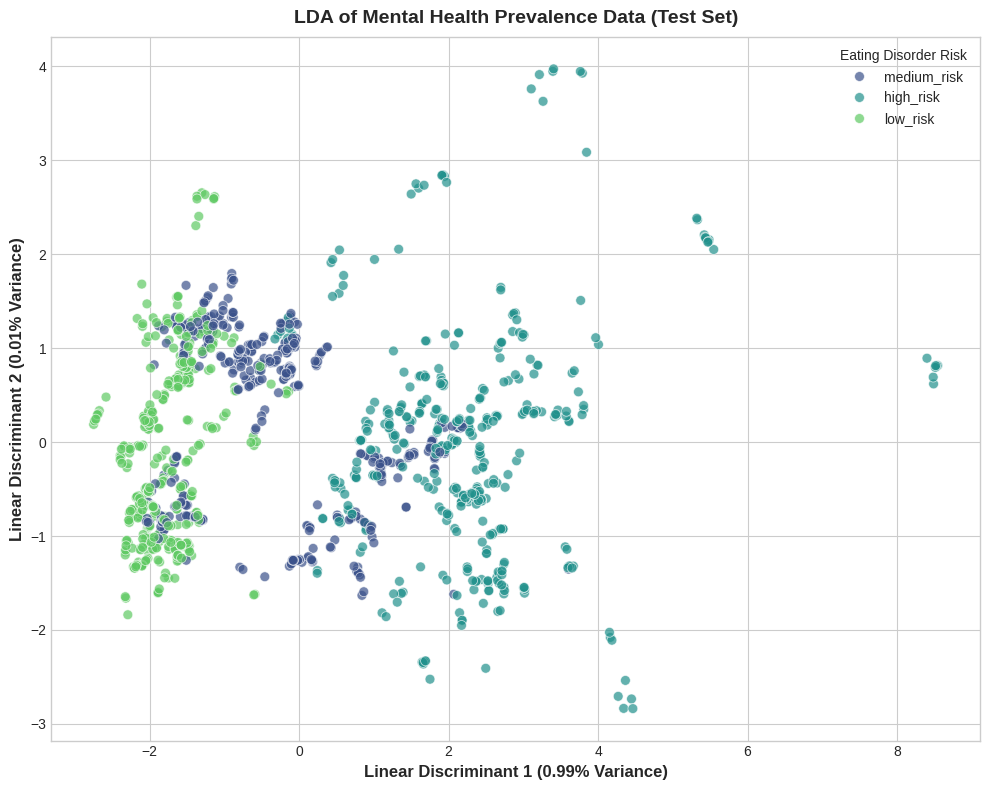
\includegraphics[scale=0.3]{figures/lda_result.png}
%         \caption{LDA}
%         \label{fig:lda}
%     \end{figure}

\section{Predicting prevalence of Eating Orders}

This section covers various prediction models used to predict the rate or prevalence of eating disorders by fitting multiple models to numerical features in the mental illness prevalence dataset [cite]. 

\subsection{GLM}
To assess the combined effect of psychiatric disorders on the prevalence of eating disorders, we constructed a generalized linear regression model (GLM) with four main independent variables: bipolar disorder, anxiety disorder, depression disorder, and schizophrenia. This multivariate approach enabled the examination of the individual effects of each factor while controlling for the presence of the remaining factors.
\begin{itemize}
    \item Dependent variable: eating disorders
    \item Independent variables: bipolar disorder, anxiety disorder, depressive disorder, schizophrenia
    \item Model type: GLM with Gaussian distribution and identity link function
\end{itemize}
All variables have significant effects on eating disorders, suggesting that each of these disorders plays an important role in predicting the prevalence of eating disorders. In particular, bipolar disorder and schizophrenia are the two strongest factors with the highest coefficients in the model.

\subsection{Neural Network}

Neural networks are constructed of multiple layers of simplified artificial neurons that sum all weighted inputs (with bias) and apply activation \( f \). This result \( y \) can then be propagated as an input in the next layer of the neural network. 

\[
y = f\left(\sum_{j=0}^{i} w_j x_j + b_j \right)
\]

Neural networks can be used for regression or classification and for predicting prevalence of eating disorders given various other disorders as input, we have one output node representing this prediction. Training of the neural network is done via backward propagation, where we effectively use the derivative chain rule [Add citation here] to adjust weights back through the neural network from the desired output node value. A simplified mental model here would be that we change the inputs by a specific amount and the output changes by a corresponding amount (slope or derivative).  

%TODO Some references to read and cite:
%  (Kuhn & Johnson, 2016, p. 34). (Kuhn & Johnson, 2016, p. 361).

    % \begin{figure}[!ht]
    %     \centering
    %     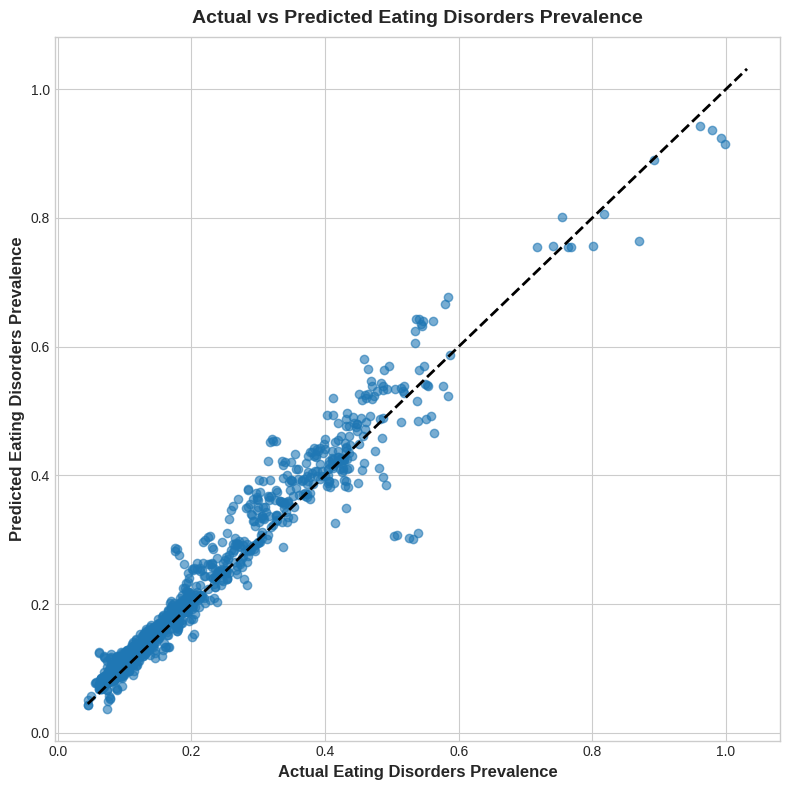
\includegraphics[scale=0.3]{figures/nn_predicted.png}
    %     \caption{Neural Network Predictions.}
    %     \label{fig:nn_pred}
    % \end{figure}
    % \begin{figure}[!ht]
    %     \centering
    %     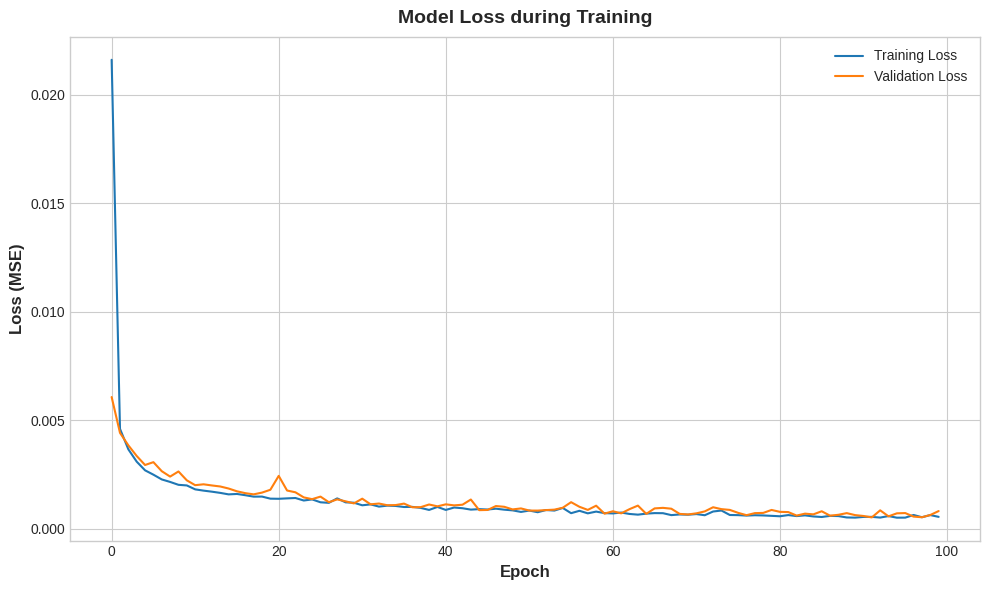
\includegraphics[scale=0.3]{figures/nn_model_loss.png}
    %     \caption{NN Model Loss.}
    %     \label{fig:nn_model_loss}
    % \end{figure}

\subsection{Random Forest Regressor}

The Random Forest Regressor is an ensemble learning algorithm that builds multiple decision trees and outputs the average of their predictions to estimate a continuous target variable. By averaging over many trees trained on different subsets of the data (via bootstrapping), it reduces overfitting and improves generalization. Unlike XGBoost, which builds trees sequentially and focuses on correcting errors made by previous trees, Random Forest builds trees independently in parallel. This simplicity comes with the benefit of easier interpretability and tuning, as its hyperparameters primarily control the number and depth of trees in the forest.

A simple analogy for describing the differences between decision trees (DT), random forests (RF) and XGBoost is playing a hole of golf: 
\begin{itemize}
    \item for DT you get one shot off the tee
    \item for RF you can hit many balls and pick the best one
    \item for XGBoost you can hit one ball walk up to the ball and hit it again until you get close to the hole as possible
\end{itemize}

    % \begin{figure}[!ht]
    %     \centering
    %     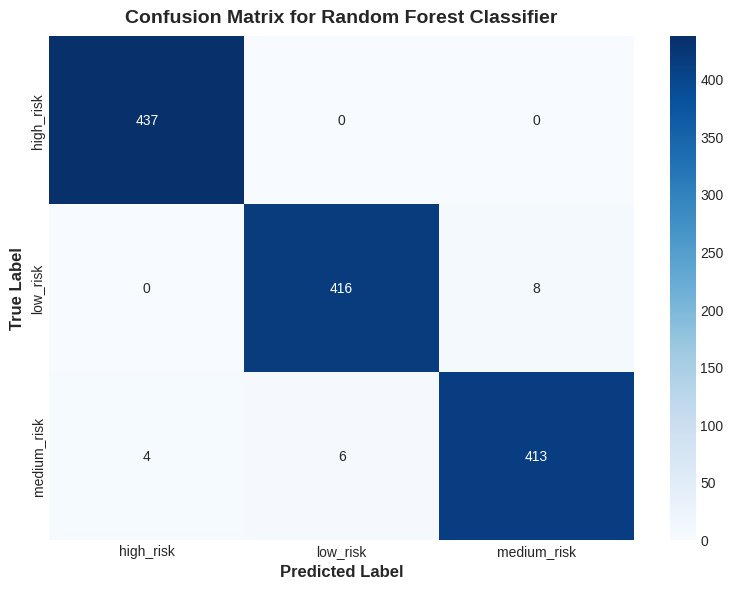
\includegraphics[scale=0.3]{figures/rnd_conf_matric.png}
    %     \caption{Random Forest Confusion Matrix.}
    %     \label{fig:rf_confusion_matrix}
    % \end{figure}
    % \begin{figure}[!ht]
    %     \centering
    %     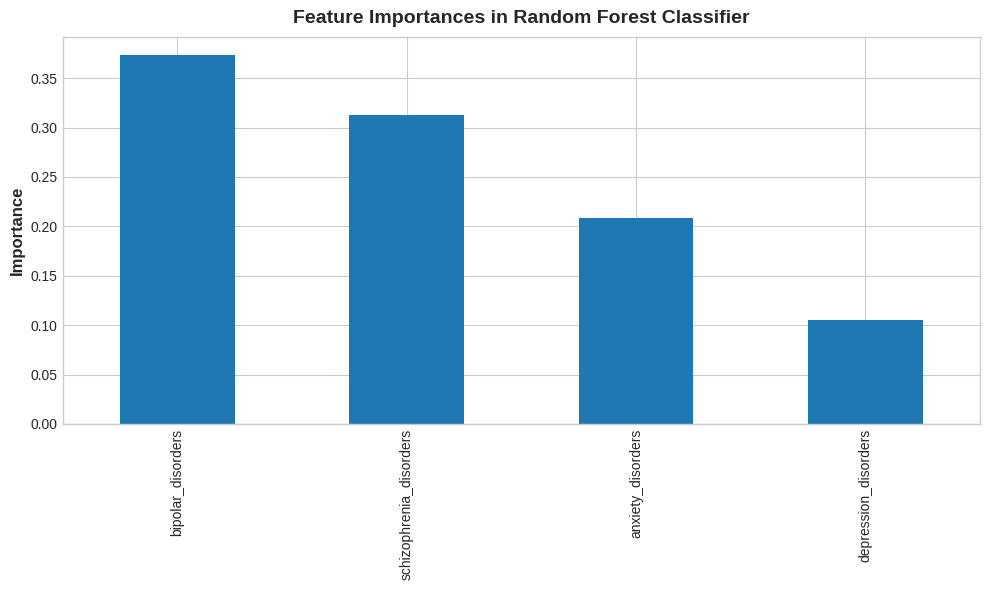
\includegraphics[scale=0.3]{figures/rnd_feature_importance.png}
    %     \caption{Random Forest Feature Importance}
    %     \label{fig:rf_importance}
    % \end{figure}
    % \begin{figure}[!ht]
    %     \centering
    %     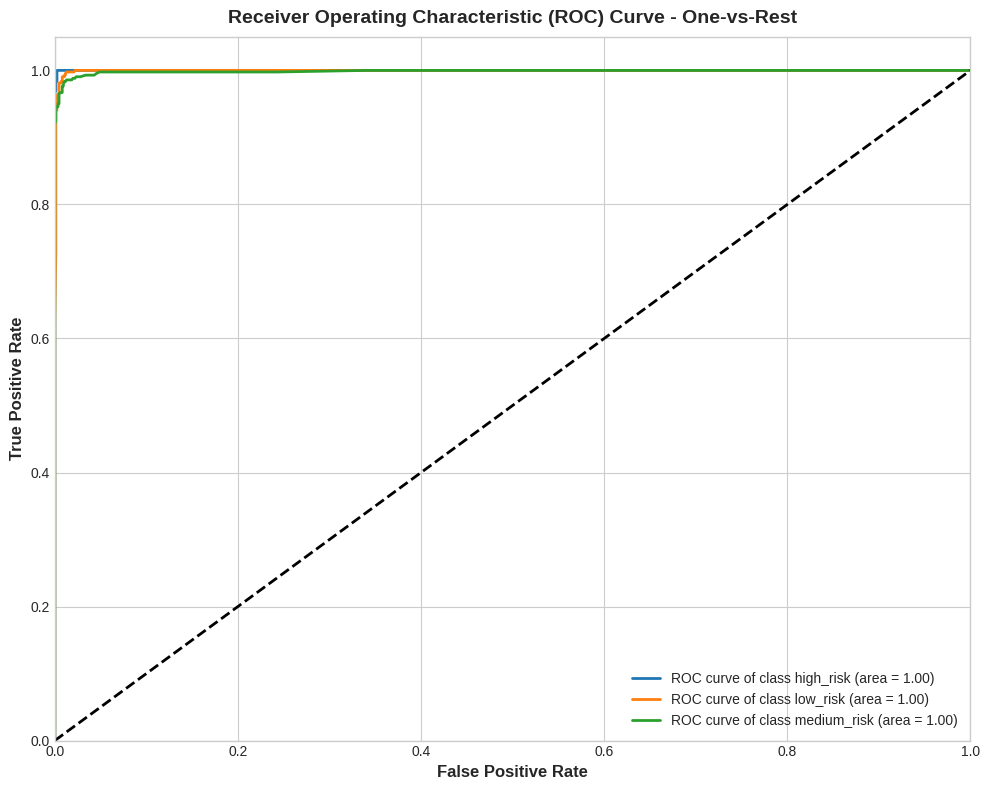
\includegraphics[scale=0.3]{figures/rnd_roc_curve.png}
    %     \caption{Random Forest ROC Curve.}
    %     \label{fig:rf_roc}
    % \end{figure}
    

\subsection{K-Nearest Neighbours}

K-Nearest Neighbours (KNN) is a supervised learning algorithm that predicts the output for a given data point by looking at the outputs of the K most similar instances in the training set. Similarity is typically measured using a distance metric like Euclidean distance. In regression, the predicted value is usually the average of the target values of these K neighbours. KNN is non-parametric, meaning it makes no assumptions about the underlying data distribution, and it can model complex relationships with sufficient data.

\begin{algorithm}
    \caption{K-Nearest Neighbours (KNN) Regression}
    \label{algo:knn}
    \begin{algorithmic}[1]
        \Require{$\mathbf{X} = \{x_1, x_2, \ldots, x_n\}$ (training features), $\mathbf{y} = \{y_1, y_2, \ldots, y_n\}$ (target values), $x_{\text{query}}$ (query point), $K$ (number of neighbours)}
        \Ensure{Predicted value $\hat{y}$ for $x_{\text{query}}$}
        \Statex
        \Function{KNNRegression}{$\mathbf{X}, \mathbf{y}, x_{\text{query}}, K$}
        \For{$i \gets 1$ to $n$}
            \State $d_i \gets \|x_i - x_{\text{query}}\|$
            \Comment Compute distance from query point
        \EndFor
        \State Identify indices $I$ of $K$ nearest neighbours with smallest $d_i$
        \State $\hat{y} \gets \frac{1}{K} \sum_{i \in I} y_i$
        \Comment Predict as average of $K$ nearest target values
        \State \Return $\hat{y}$
        \EndFunction
    \end{algorithmic}
\end{algorithm}

\subsection{Support Vector Regressor}

Support Vector Regression (SVR) is a supervised learning algorithm derived from Support Vector Machines (SVMs) (\cite{svr}), but designed for predicting continuous outcomes rather than classifying categories. In the context of predicting outcomes such as the severity or risk of eating disorders, SVR constructs a function that fits the data within a specified margin of tolerance, rather than attempting to classify it into discrete groups. The algorithm seeks a regression hyperplane that minimizes deviations beyond a pre-defined threshold (epsilon), while simultaneously ensuring that the model remains as flat (simple) as possible. The support vectors in this context are the data points that lie on or outside the margin and influence the position of the regression line \cite{kuhn2016}.

To capture complex, nonlinear relationships between features and the target variable, we apply the Radial Basis Function (RBF) kernel. This kernel function implicitly maps the input data into a higher-dimensional feature space, allowing the SVR model to learn nonlinear patterns without explicitly performing the transformation. This flexibility is especially useful when the input features have intricate interactions. To ensure the training and testing datasets maintain representative distributions, we use stratification during data splitting.
    
\section{Results – Model Analysis}
\label{sec:results}

\textbf{Linear regression} analysis result showed that all three psychiatric disorders, bipolar disorder, anxiety disorder, and schizophrenia, had a positive linear relationship with the prevalence of eating disorders. Among them, bipolar disorder showed the strongest predictive power with a coefficient of $R^2$=0.46, followed by anxiety disorder (0.35) and schizophrenia disorder (0.25). Despite the different levels of association, all three models had a low mean square error (MSE) of only 0.01, indicating that the model had high predictive accuracy when using standardized data. These results confirm that psychiatric disorders, especially bipolar disorder, are important predictors of eating disorder prevalence in the population.

Table~\ref{tab:model_results} shows evaluation metrics for five regression models: GLM, K-Nearest Neighbors, Neural Network, Random Forest, and Support Vector Regressor. For each model we calculate $R^2$ and mean squared error (MSE) scores for train and test predictions. We also calculate a 95\% confidence intervals (CI) for the test $R^2$ score where applicable, and $p$-values highlighting the differences in performance relative to the Random Forest Regressor.

The \textbf{Generalized Linear Model} using a train-test split indicates that all mental health disorders analyzed have a statistically significant impact on eating disorders:
\begin{itemize}
    \item \textbf{Bipolar disorder} shows the strongest effect, with a coefficient of +0.4156,
    \item \textbf{Schizophrenia disorder} follows closely with a strong positive effect of +0.3912,
    \item \textbf{Anxiety disorder} has a moderate positive effect (+0.1312),
    \item \textbf{Depression disorder} also contributes positively, though the effect is smaller (+0.0346).
\end{itemize}
All predictor variables had significant effects on eating disorders, and it was concluded that these disorders can predict the prevalence of eating disorders.The $R^2$ value on the test set was 0.68, and on the training set was 0.65, indicating that the model has strong explanatory power. The 95 percent confidence interval on the test set was between (0.6526 and 0.7017), indicating the high stability of the model. The mean square error (MSE) was 0.0006 on the training set and 0.00064 on the test set, indicating that the model predicted accurately and with slight bias.

The \textbf{Random Forest Regressor} was the best overall performing model and achieved the highest test $R^2$ score (0.9950) and the lowest test MSE (0.000101). Its 95\% confidence interval for the test $R^2$ \([0.9908, 0.9984]\) was also the tightest amoung all models (this result strongly indicates consistent generalization).

The \textbf{K-Nearest Neighbors Regressor} also performed well and achieved a test $R^2$ of 0.9893 and a narrow confidence interval \([0.9793, 0.9966]\), showing reliable generalization. 

The \textbf{Neural Network} model yielded a test $R^2$ of 0.9156 and a test MSE of 0.001686. While this performance was weaker than the tree-based models, it was run for 100 iterations and demonstrated reasonable accuracy. The $p$-value ($2.18 \times 10^{-11}$) indicates a statistically significant difference in the performance relative to the  Random Forest regressor model.

The \textbf{Support Vector Regressor} showed the lowest predictive performance with a test $R^2$ of 0.8037 and a test MSE of 0.003922. Furthermore the confidence interval \([0.7742, 0.8295]\) showed the model had a lower stability and accuracy.

\begin{table}[h!]
\centering
\caption{Model Evaluation Metrics with Confidence Intervals and Significance Testing}
\label{tab:model_results}
\begin{tabular}{lcccccc}
\toprule
\textbf{Model} & $R^2_{\text{train}}$ & $R^2_{\text{test}}$ & 95\% CI & MSE$_{\text{train}}$ & MSE$_{\text{test}}$ & $p$-value \\
\midrule
GLM & 0.65 & 0.68 & [0.653, 0.702] & 0.0067 &  0.0064 & -- \\
K-Nearest Neighbors & 0.9952 & 0.9893 & [0.9793, 0.9966] & 9.1e-05 & 2.1e-04 & -- \\
Neural Network & 0.9286 & 0.9156 & -- & 1.4e-03 & 1.7e-03 & 2.18e-11 \\
\textbf{Random Forest} & \textbf{0.9995} & \textbf{0.9950} & [\textbf{0.9908}, \textbf{0.9984}] & \textbf{1.0e-05} & \textbf{1.0e-04} & \textbf{6.05e-03} \\
Support Vector Regressor & 0.8016 & 0.8037 & [0.7742, 0.8295] & 3.8e-03 & 3.9e-03 & < 1e-40 \\
GLM & - & 0.085 & - & < mse & < mse & < 0.001 \\
\bottomrule
\end{tabular}
\end{table}

In summary: as shown in Table~\ref{tab:model_results}, the \textbf{Random Forest Regressor} achieves the highest performance, with the lowest test MSE (0.000101) and the highest test $R^2$ (0.9950). 
This on the surface indicates good generalization ability. The \textbf{K-Nearest Neighbors Regressor} also performs well, albeit with a slightly higher test MSE error. The neural network model showed some larger MSE and could benefit from larger number of iterations or alternative network architecture (which we will leave to future work).

\subsection{Relationship between the quality of healthcare
measured by the Universal Health Coverage (UHC) Index and Depression across countries}

\begin{table}[h!]
\centering
\caption{Yearly Correlation and Regression Results for UHC and Depression Rates}
\label{tab:uhc_depression_results}
\begin{tabular}{|l|c|c|c|c|c|c|}
\hline
\textbf{Year} & \textbf{Pearson $r$} & \textbf{$p$-value} & \textbf{95\% CI for $r$} & \textbf{Regression Slope ($\beta$)} & \textbf{95\% CI for $\beta$} & \textbf{$R^2$} \\
\hline
2000 & -0.32 & $<.001$ & -- & -0.0151 & [$-0.022$, $-0.008$] & 0.104 \\
2005 & -0.37 & $<.001$ & -- & -0.0165 & [$-0.023$, $-0.010$] & 0.135 \\
2010 & -0.40 & $<.001$ & -- & -0.0198 & [$-0.027$, $-0.013$] & 0.163 \\
2015 & -0.45 & $<.001$ & -- & -0.0221 & [$-0.029$, $-0.015$] & 0.205 \\
2017 & -0.45 & $<.001$ & -- & -0.0224 & [$-0.029$, $-0.016$] & 0.200 \\
2019 & -0.46 & $<.001$ & -- & -0.0228 & [$-0.030$, $-0.016$] & 0.208 \\
\textbf{Overall} & \textbf{-0.41} & \textbf{$<.001$} & \textbf{[$-0.53$, $-0.28$]} & -- & -- & -- \\
\hline
\end{tabular}
\end{table}

Table \ref{tab:uhc_depression_results} presents a comprehensive analysis of annual data from 2000 to 2019, highlighting Pearson correlation coefficients, regression slopes, and $R^2$ values that investigate the relationship between the Universal Health Coverage (UHC) Index and rates of depression across various countries. The analysis reveals that, in each year examined, higher UHC scores correlate with lower national depression rates. The negative regression coefficients indicate that increases in health coverage are consistently associated with modest yet significant decreases in the prevalence of depression. These findings provide robust evidence of a stable inverse relationship between access to healthcare and mental health outcomes on a global scale.

\subsubsection{Case Study}
\begin{table}
\centering
\caption{Comparison of Mean UHC Index and Depression Rates: United States and Sweden}
\label{tab:mean_uhc}
\begin{tabular}{|l |l |l|}\hline
Country & Mean UHC Index & Mean Depression Rate (\%) \\\hline

\textbf{Sweden} & 80.5 & 4.17 \\\hline
\textbf{United States} & 83.0 & 4.43 \\\hline
\textbf{Difference} & +2.5 & +0.27 \\ \hline

\end{tabular}

\end{table}

Table \ref{tab:mean_uhc} presents the average UHC index and mean depression rates for the United States and Sweden. While the United States has a slightly higher UHC index, Sweden exhibits a lower average depression rate. This pattern suggests that, although broader health coverage is essential, additional factors, such as the quality of care, access to mental health services, and broader social support, likely contribute to national mental health outcomes.
\section{Conclusions and Recommendations}
\label{sec:con}

This research employed a combination of linear regression, generalized linear models (GLM), and advanced machine learning algorithms, including artificial neural networks, random forests, K-nearest neighbors (KNN), and support vector regression (SVR), to analyze the relationship between mental disorders and the prevalence of eating disorders. By applying correlation matrices, covariance matrices, and regression analysis on standardized data, the study not only identified the relevant factors but also evaluated the predictive power of each model.
The application of a training and testing set separation strategy ensures objectivity and highlights the generalizability of the models when applied to real-world data. The results of the study indicate that mental disorders, especially bipolar disorder and schizophrenia, are strong predictors of the prevalence of eating disorders. Models such as GLM and Random Forest showed high predictive performance and good explanatory power, while neural networks provided reasonable complementary insights. The consistency of statistical indicators, such as correlation, $R^2$, MSE, and confidence intervals, strengthened the confidence in the findings.

In addition, extending the analysis to data on universal health coverage (UHC) and national depression prevalence provides a more comprehensive context for understanding the influence of health system factors on community mental health. Therefore, research contributes not only a way in which further to understand the link between mental disorders and eating disorders but also serves as a framework for applicable public health policy and intervention approaches for the prevention and treatment of eating disorders, eating behaviors, and mental health. This research also serves as a foundation for future studies to develop and deploy practical and widely useful predictive models for mental health care.

While exploring the link between Universal Health Coverage and depression, this analysis concludes that countries with better healthcare systems tend to have lower depression rates (World Health Organization, 2022). However, when focusing on a specific case study comparing the healthcare systems of the United States and Sweden, the findings show that even though the United States has a higher UHC index, it still has a higher rate of depression. These results suggest that additional factors, including the quality of care, access to mental health services, and broader social conditions, play a crucial role in determining national mental health outcomes (Patel et al., 2018).

\subsection{Future work}

Future research should explore how additional factors, such as income, education, and social support, interact with health coverage to impact depression rates (Allen et al., 2014; Patel et al., 2018). It may also be beneficial to analyze policy variations, monitor changes within countries over time, or concentrate on specific subgroups to gain a clearer understanding of which populations derive the most benefit from expanded healthcare (World Health Organization, 2022). Investigating these areas could offer a more comprehensive insight into the connections between health systems and mental health outcomes.


\printbibliography

\appendix % Start of the appendix section

\section{Notebook Appendix} % Title for your appendix
\includepdf[pages=-]{mental_main_report}
%\includepdf{mental_main_report} % Include your notebook PDF

\end{document}
